\documentclass{book}
\usepackage[allcolors=true]{hyperref}
\usepackage{graphicx}
\usepackage{amsmath,amsfonts,amsthm,amssymb}
\usepackage{mathabx}
\usepackage{wasysym}
\usepackage{caption}
\usepackage{multirow}
\usepackage{physics}
\usepackage{tikz}
\usepackage{cleveref}
\usepackage{pgfplotstable}
\usepackage{siunitx}
\usepackage{wrapfig}
\usepackage{subfiles}
\usepackage{systeme}
\usepackage{bm}
\usepackage{xcolor}
\usepackage[french]{babel}
\usepackage{titlesec}
\usepackage{lmodern}
\usepackage{braket}
\usepackage{chngcntr}
\usepackage{geometry}
\usepackage[tc]{titlepic} % page de garde
\geometry{
     a4paper,
    total={170mm,257mm},
    left=20mm,
    top=20mm,
 }

\numberwithin{equation}{part}
\counterwithin*{section}{part}

\pgfplotsset{width=10cm,compat=1.16}
\newcommand{\cst}{\text{c}^{\text{\scriptsize ste}}}
\newcommand{\ddx}{\dfrac{\textrm d ^2 x}{\textrm d t^2}}
\newcommand{\ti}{\times}
\newcommand{\h}{\hbar}
\renewcommand{\d}{\mathrm{d}}
\newcommand{\dx}{\mathrm{d}x}
\newcommand{\dy}{\mathrm{d}y}
\newcommand{\dz}{\mathrm{d}z}
\newcommand{\dt}{\mathrm{d}t}
\newcommand{\dxp}{\mathrm{d}x'}
\newcommand{\dyp}{\mathrm{d}y'}
\newcommand{\dzp}{\mathrm{d}z'}
\newcommand{\dtp}{\mathrm{d}t'}
\newcommand{\dvx}{\mathrm{d}\vec x}
\newcommand{\dvxp}{\mathrm{d}\vec x'}
\newcommand{\ch}{\mathrm{ch}}
\newcommand{\sh}{\mathrm{sh}}
\renewcommand{\th}{\mathrm{th}}
\newcommand{\tg}{\mathrm{tg}}
\newcommand{\C}{\textbf{C} }
\newcommand{\Cpp}{\textbf{C}++ }
\newcommand{\ud}[3]{{#1}^{#2} _{\; {#3} }}
\newcommand{\du}[3]{{#1}_{#2} ^{\; {#3} }}
\renewcommand{\dd}[3]{{#1}_{#2} _{\; {#3} }}
\newcommand{\uu}[3]{{#1}^{#2} ^{\; {#3} }}
\renewcommand{\thepart}{\arabic{part}}


\titleformat{\paragraph}
{\normalfont\normalsize\bfseries}{\theparagraph}{1em}{}
\titlespacing*{\paragraph}
{0pt}{3.25ex plus 1ex minus .2ex}{1.5ex plus .2ex}

\renewcommand{\thepart}{\Roman{part}} 


\newtheorem{theorem}{Théorème}[section]
\newtheorem{definition}[theorem]{Définition}
\newtheorem{lemma}[theorem]{Lemme}
\newtheorem{Property}[theorem]{Proposition}
\newtheorem{corollary}[theorem]{Corollaire}
\newtheorem{remark}[theorem]{Remarque}
\newtheorem*{preuve}{Preuve}
\newtheorem{reminder}[theorem]{Rappel théorique}
\newtheorem{exemple}[theorem]{Exemple}

\renewcommand\qedsymbol{$\blacksquare$}

\setcounter{tocdepth}{2}

\usepackage{enumitem}

%%% Début ajouts Sami
% Nouvelles couleurs (BG = Background)
\definecolor{bleu}{RGB}{14, 68, 175}
\definecolor{BGbleu}{RGB}{222, 233, 255 }
\definecolor{BGorange}{RGB}{255, 216, 154}
\definecolor{BGgris}{RGB}{222,230,230}
\definecolor{rouge}{RGB}{201, 0, 0}
\definecolor{vert}{RGB}{14, 137, 0}
\newcommand\rouge[1] {{\color{rouge}{#1}}}
\newcommand\bleu[1] {{\color{bleu}{#1}}}
\newcommand\green[1]{{\color{vert}{#1}}}

% Boites
\newcommand\bg[2]{
\begin{center}
\fcolorbox{white}{BGgris}{\parbox{.9\linewidth}{\begin{large} \textit{#1} \end{large} \\

#2 }}
\end{center}}
% Boite d'alerte
\definecolor{BGorange}{RGB}{255, 216, 154}
\newcommand\probleme[1]{
\begin{center}
\fcolorbox{white}{BGorange}{\parbox{.9\linewidth}{\begin{large} \textbf{Problème} \end{large} \\

#1}}
\end{center}}

% boite bleue
\newcommand\bb[1]{
\begin{center}
\fcolorbox{black}{BGbleu}{\parbox{\textwidth}{ 
\begin{Large}
\begin{center}
#1
\end{center}
\end{Large}
}}
\end{center}}

\setlength{\fboxsep}{1em} % espace entre le bord d'une boite et le texte dedans


% Commande spéciale pour wrap facilement
%% Wrapping %%
\newcommand\wrap[4]{\begin{wrapfigure}[#1]{#2}{#3\textwidth}
    #4
    \end{wrapfigure}}
%%% Fin ajouts Sami

\title{\textbf{PHYS-F203 - Introduction à la Mécanique Quantique} \\ \textit{Basé sur les notes de Prof. $\href{mailto:serge.massar@ulb.be}{\text{Massar Serge}}$}}
\author{$\href{mailto:juian.moeil@ulb.be}{\text{Moeil Juian}}$ \and $\href{mailto:sami.abdul.sater@ulb.be}{\text{Abdul Sater Sami}}$ \and $\href{mailto:anais.defossez@ulb.be}{\text{Defossez Anais }}$}
\date{\textbf{Année académique 2020-2021}}

\begin{document}


%% Page de garde : https://tex.stackexchange.com/questions/10130/use-the-values-of-title-author-and-date-on-a-custom-title-page pour l'utilisation des variables, et @SAS pour la page de garde
\makeatletter
\begin{titlepage}
    \centering
    \huge{\@title} \\
    \vspace{1cm}
    \@date \\
    \vspace{1cm}
    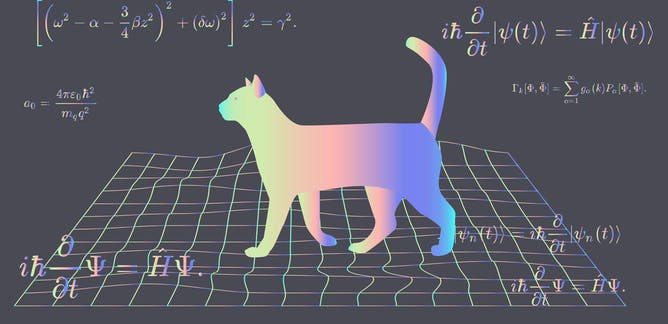
\includegraphics[scale=0.65]{Images/cat.jpg} \\
    \vspace{1cm}
    \begin{minipage}{\linewidth}
        \begin{minipage}{0.45\linewidth}
            \begin{center}
                
\includegraphics[scale=0.2]{Images/sciences.png} 
            \end{center}
        \end{minipage}
        \begin{minipage}{0.5\linewidth}
            \begin{flushright}
                \begin{tabular}{r}
                    Auteurs \\
                    \hline
                    \href{mailto:juian.moeil@ulb.be}{Moeil Juian} \\
                    \href{mailto:anais.defossez@ulb.be}{Defossez Anais} \\
                    \href{mailto:sami.abdul.sater@ulb.be}{Abdul Sater Sami}
                \end{tabular}
            \end{flushright}
        \end{minipage}
    \end{minipage}
    \\
    \vfill
    
\includegraphics[scale=0.5]{Images/ULB.jpg} \\
\end{titlepage}
\makeatother

\chapter*{Avant-propos}
\textit{Ce document a été initialement conçu par Juian Moeil pour contenir les notes de cours de Pr. Serge Massar, pour le cours \href{https://www.ulb.be/fr/programme/phys-f203}{PHYS-F203} dispensé à l'ULB durant l'année académique 2020-2021. Sami et Anais ont rejoint l'aventure durant l'été 2021 pour le mettre à jour : approfondir le contenu et y faire contenir des réflexions et interprétations qui ne viennent pas explicitement des notes manuscrites. \\ \\
Certaines parties du chapitre 2 sont inspirées de \href{https://www.ulb.be/fr/programme/phys-h200}{PHYS-H200}, \textit{Physique Quantique et Statistique}, dispensé par Pr. Jean-Marc Sparenberg. \\ \\
Ces notes sont donc l'oeuvre de compréhension et d'interprétation d'étudiants, qui n'ont aucunement la prétention de ne pas commettre d'erreur : d'orthographe, de grammaire, voire pire, physique. N'hésitez donc pas à contacter Juian, Anais, ou Sami, pour toute remarque (adresse e-mail cliquable en page de garde).
} \\

Le document est structuré comme suit : la partie 1 présente les fondements et le formalisme de la Mécanique Quantique. En commençant par le principe d'incertitude d'Heisenberg (chapitre \ref{chap:chap1}) et l'observation de la dualité onde-particule (chapitre \ref{chap:chap2}). Ce dernier chapitre aboutit sur l'équation de Schrödinger (chapitre \ref{chap:chap3}). Ensuite, il est question d'aborder le formalisme et les postulats de la Mécanique Quantique. \\

La partie 2 concernerait les applications de la Mécanique quantique, et contient, dans la numérotation de S. Massar, les chapitres 5 à 8 compris. \\

Les chapitres 1 à 3 ont été revus en profondeur. Le chapitre 4 est en cours de (profonde) révision, et les chapitres au-delà contiennent une retranscription des notes manuscrites de S. Massar et nécessitent révision (et approfondissement). \\

Le symbole $\doteq$ est employé pour dire "par définition". Les vecteurs $\bm{x}$ sont indiqués en gras.


\newpage
\tableofcontents

\part{Fondements et formalisme de la Mécanique Quantique}
\subfile{Chapitre 1/chapitre1.tex}  %   Incertitude
\newpage
\subfile{Chapitre 2/chapitre2.tex}  %   Fondements 
\newpage
\subfile{Chapitre 3/chapter3.tex}  %   Equation de Schrodinger
\newpage
\subfile{Chapitre 4/chapitre4.tex}  %   Formalisme
\newpage
<<<<<<< HEAD
=======
\begin{abstract}
\textit{Ces notes traitent de l'interprétation de Copenhague de la Mécanique Quantique, telle qu'enseignée dans le cadre du cours $\href{https://www.ulb.be/fr/programme/phys-f203}{\text{PHYS-F203}}$ en 2020-2021 à l'Université Libre de Bruxelles.} \end{abstract}
\begin{remark}
    Le symbole $\doteq$ est employé pour dire "par définition". Les vecteurs $\bm{x}$ sont indiqués en gras.
\end{remark}
>>>>>>> main

\part{Application de la Mécanique quantique}
\subfile{Chapitre 5/chapitre5.tex}
\newpage
\subfile{Chapitre 6/chapitre6.tex}  % Opérateurs X et P
\newpage
\subfile{Chapitre 7/Chapitre7.tex}  % Oscillateur harmonique

\newpage
\subfile{Annexe/annexe.tex}         % Notions mathématiques, etc.

\end{document}